\documentclass[preprint]{aastex} %double-column, single-spaced document:
%\documentclass[iop,floatfix]{emulateapj} 

\usepackage[breaklinks,colorlinks,urlcolor=blue,citecolor=blue,linkcolor=blue]{hyperref}
\usepackage{graphicx}
\usepackage{apjfonts}
\usepackage{enumerate}
\usepackage{amsmath,amssymb}
\usepackage{bm}
\usepackage[usenames,dvipsnames,svgnames,table]{xcolor} 
\usepackage[utf8]{inputenc}

%version-control tagging based off of github.com/bd-j/speccal
%%% This file is generated by Makefile.
\newcommand{\githash}{9a841bd}\newcommand{\gitdate}{2014-12-09}\newcommand{\gitauthor}{Ian Czekala}

\newcommand{\prob}{{\rm prob}}
\newcommand{\qN}{\{q_i\}_{i=1}^N}
\newcommand{\qM}{\{q_{im}\}_{i=1,m=0}^{N,M}}
\newcommand{\yN}{\{y_i\}_{i=1}^N}
\newcommand{\vt}{\vec{\theta}}
\newcommand{\vg}{\vt_{\star, {\rm grid}}}
\newcommand{\vpp}{\vt_{\star, {\rm post}}}
\newcommand{\vstar}{\vt_{\star}}
\newcommand{\finst}{f_{\lambda, {\rm inst}}}
\newcommand{\fsynth}{f_{\lambda, {\rm synth}}}
\newcommand{\vN}{\vt_{\rm N}}
\newcommand{\vc}{\vec{c}}
\newcommand{\fM}{ \vec{{\bm M}}}
\newcommand{\fMi}{M_i}
\newcommand{\fD}{ \vec{{\bm D}}}
\newcommand{\fDi}{D_i}
\newcommand{\fR}{ {\bm R}}
\newcommand{\dd}{\,{\rm d}}
\newcommand{\trans}{\mathsf{T}}
\newcommand{\Z}{[{\rm Fe}/{\rm H}]}
\newcommand{\A}{[\alpha/{\rm Fe}]}
\newcommand{\matern}{Mat\'{e}rn}

\newcommand{\todo}[1]{ \textcolor{Blue}{\\TODO: #1}}
\newcommand{\comm}[1]{ \textcolor{Red}{SA: #1}}


%% Nomenclature guide
%%%%%%%%%%%%%%%%%%%%%
% * collections of synthetic spectra are generically called ``libraries.'' The term 
% ``grid'' is used when referring specifically to the spacing of spectral parameters
% in the library 

\shorttitle{Spectroscopic inference}
\shortauthors{Czekala et al.}

\begin{document}

\graphicspath{{figs/}}

\title{A Method for the spectroscopic inference of fundamental stellar parameters}
\author{\today{}\\
\medskip
Ian~Czekala\altaffilmark{1} et al.
%Author2\altaffilmark{2},
}

\altaffiltext{1}{Harvard-Smithsonian Center for Astrophysics, 60 Garden Street 
 MS 10, Cambridge, MA 02138}
%\altaffiltext{2}{Institution 2}
\email{iczekala@cfa.harvard.edu}

\section{Introduction}
\begin{itemize}
  \item Where our technique fits in the ecosystem of stellar methods.
  \item Applicable to any kind of spectrum (long-slit, echelle, infrared,
    flux-calibrated or not)
  \item Examples of fields where accurate and unbiased stellar parameters are
    crucial. Exoplanets. T Tauri stars.
\end{itemize}

\section{Method}

A single spectrum provides a wealth of information that can be used to infer the fundamental properties of a star: effective temperature $T_{\rm eff}$, surface gravity $\log g$, and metallicity $\Z$; together $\vg$. We wish to extract the maximal amount information from a given spectrum while also recognizing the limitations imposed by our stellar model and exposing any degeneracies between the parameters.  For example, if we model a large range of the spectrum at once (e.g., the full optical range at high resolution), then we must explicitly account for any covariances and biases introduced by improper calibration or inaccuracies in the model spectrum. We present a generative model which uses a synthetic stellar library as a backend and apply post-processing techniques to mimic the observed spectrum as a function of several stellar parameters and calibration parameters in order to determine the best fit. By forward modelling the data spectrum in a Bayesian framework, our modular approach can easily incorporate additional calibration artifacts and stellar complexity (e.g., veiling or Zeeman splitting) while still being true to the limitations of the dataset.  This data driven approach will enable us to learn how the underlying synthetic models may be improved and refined in an iterative manner.  

The roadmap for our method is as follows.
 First, for a given set of fundamental stellar parameters $\vg$, we generate a synthetic
 spectrum by interpolating from a grid of synthetic spectra (\S\ref{subsec:synthetic}). 
Then, we post-process the interpolated spectrum for realism by using additional
 parameters to describe Doppler shift, projected rotational velocity,
 interstellar extinction, and residual flux calibration errors
 (\S\ref{subsec:postprocess}). 
We perform a pixel-by-pixel comparison of the generated spectrum with the
 data spectrum using a prescribed likelihood function
 (\S\ref{subsec:likelihood}) and a parametric treatment of the covariance
 between pixel residuals (\S\ref{subsec:covariance}). 
We use a Markov chain Monte Carlo (MCMC) Gibbs sampler to numerically explore
the posterior probability density and determine constraints on the stellar
and nuisance parameters (\S\ref{subsec:MCMC}). 
The benefit of our method is that it provides robust estimates of the stellar and nuisance
parameters with well-quantified uncertainties and parameter degeneracies. 
Our parameterization of the covariance between pixel residuals also yields a means to identify
 and quantify the key discrepancies between the data and model, and provides a path forward to 
 improve the stellar models in an iterative fashion (\S\ref{subsec:learning}).
 \todo{I really want to overload the word ``covariance'' and use it to describe both the covariance between $T_{\rm eff}$ and $\log g$ as well as the covariance structure of the pixel residuals themselves. However I think this might be confusing so I am using ``degeneracies'' for the former and reserving ``covariance'' for the later.}

\subsection{Synthetic Model Spectra}
\label{subsec:synthetic}
Many methods exist to generate a synthetic model of a stellar spectrum. Generally, when
a high quality spectrum is needed for a specific set of stellar parameters, one
runs a stellar atmosphere and radiative transfer code to synthesize the
spectrum. Unfortunately, it is computationally expensive to accurately generate
a spectrum over a wide range of wavelengths, and so these codes are generally
employed to generate libraries of stellar spectra, which exist over a range of
$\vg$ at specified points on a regular grid, typically covering the main sequence of stellar
types. Several high-quality libraries of synthetic spectra now exist
(\citealt{hwd+13}, Kurucz, and more are being developed for GAIA).  

In a forward-modelling approach, which may make many calls to generate a
spectra of varying $\vg$, it is currently computationally impractical to
iterate the structure of the stellar atmosphere and then run the stellar
synthesis for each call of $\vg$.  Some methods compromise by taking a halfway
approach, whereby a precomputed library of stellar atmospheres is interpolated
for a given $\vg$, and then a simple radiative transfer code is run to
synthesize a spectrum (e.g.  SME; \citealt{vp96}). This technique has the
advantage that interpolating atmospheres and then running the spectral
synthesis for each $\vg$ might be more accurate than directly interpolating
synthetic spectra. However, if a large region of wavelength is required at high
resolution, then the synthesis step will be slow.  A different approach might
be instead to eschew forward modelling (and thus repeated synthesis or grid
interpolation) of the spectra entirely and evaluate the posterior probability
density only at the grid points of the spectral library.  Then, these discrete
samples of the posterior density can be interpolated to find the posterior
surface and draw confidence intervals on the parameters (e.g. SPC;
\citealt{blj+12}). However, the difficulty with this approach is that the
parameter uncertainty might be smaller than the grid spacing, and then
interpolation will not properly capture degeneracies between parameters.

Because we desire a generative model of the spectra without the added
complexity or computational overhead of running a stellar synthesis, we opt to
use a \todo{Implement a more accurate but still fast interpolator for the grid.
Likely this will be a combination of using splines to pre-interpolate a finer
grid (~20 K, 0.1 dex spacing in gravity and metallicity and then doing linear
interpolation off of this new grid during the actual MCMC run. It will be described here.} However, the
techniques we develop in this paper to account for and parameterize the
correlated, systematic pixel residuals are generally applicable to spectra fit
by any of these methods.


\begin{figure*}[!htb]
\begin{center}
  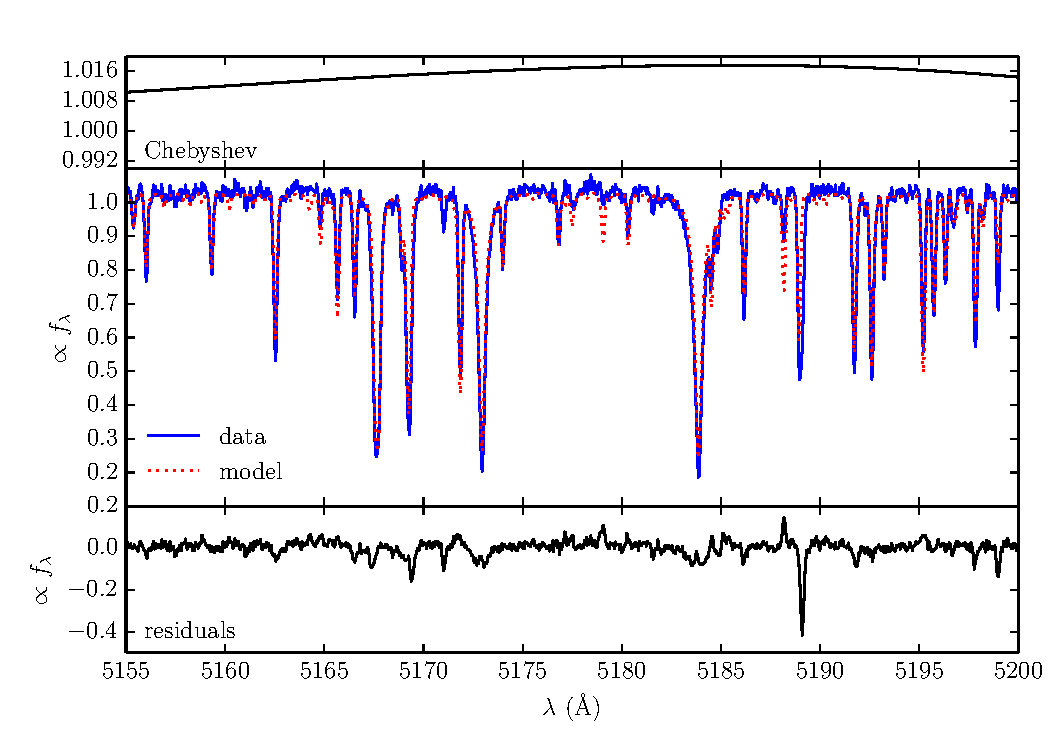
\includegraphics[width=0.85\textwidth]{figs/model_data.pdf}
  \caption{\textbf{Top}: Chebyshev polynomial which multiplies the model spectrum
   to account for inaccuracies in the flux-calibration. 
  \textbf{Middle}: The data spectrum and model spectrum, after it has been
   interpolated, post-processed, and multiplied by the Chebyshev polynomial.
  \textbf{Bottom}: Residuals from the model fit. Note the large residual at
   $\lambda5189$\AA\ due to a missing opacity source from \ion{Ca}{1}.}
\label{fig:model_data}
\end{center}
\end{figure*}


\subsection{Post-Processing}
\label{subsec:postprocess}

Libraries of synthetic spectra are generally computed at high resolution ($R
 \geq $100,000), sampled with many pixels per resolution element, and do not
 include any rotational broadening or account for any instrumental effects. 
In order to transform a raw synthetic spectrum interpolated from the grid into
 one that matches the spectrum of a real star, we must post-process the spectrum
 to account for these secondary effects. 
In addition to these fundamental parameters, a star also has several observed
 properties that are a function of its kinematics, geometry, and location in our
 galaxy: projected rotational velocity $v \sin i$, line of sight velocity $v_z$,
 total extinction $A_V$, and solid angle $\Omega$. 
We call these secondary parameters $\vpp$, because we can model their effects
 on the synthetic spectra in a ``post-processing'' step by convolution with an
 appropriate kernel or multiplication with a smooth function. 
Together, we call $\vstar = \{\vg, \vpp\}$.

The projected rotational velocity of the star, parameterized by $v \sin i$,
broadens spectral line profiles and is mathematically described by convolution
with a specific kernel \citep[Equation 18.14]{gra08}. UV, optical, and infrared
spectra are acquired using a spectrograph which disperses light onto a CCD,
defining a specific resolution and sampling rate for the spectrum.  Because the
resolution of the spectrograph and pixel sampling are different from the
synthetic spectral library, we must convolve the raw spectrum with the line
spread function (LSF) of the instrument and resample to the exact pixels of the
CCD. In wavelength space, the $v \sin i$ and LSF operations are represented by
the convolution of the synthetic spectrum with these two kernels.  Using the
convolution theorem, we can rewrite these convolutions as multiplications in
Fourier space.  In order to use the fast Fourier transform (FFT) with discrete
samples of the synthetic spectrum, we must first resample it
onto a uniform grid.  In the case of a spectrum, the natural
uniform grid is one that is equally sampled in velocity space, such there is an
equal velocity shift $\Delta v$ between pixels. This results in a wavelength
grid that is linearly sampled in the logarithm of wavelength.  Next, we
multiply the Fourier transform of the synthetic spectrum by the Fourier
transforms of the rotational velocity and line spread function kernels.
Lastly, we do an inverse FFT to transform the modified spectrum back to
wavelength space, where it is sampled at the wavelength locations of the pixels
in the detector.  When resampling the spectrum, we are careful to ensure
band-limited interpolation using splines in order to prevent introducing
non-physical high frequency structure into the spectrum.  

We scale the raw synthetic flux (often reported at the stellar surface) to an
observed flux by multiplying by the solid angle of the star, $\Omega =
R_\star^2/d^2$, where $R_\star$ is the stellar radius and $d$ is the distance
to the star from earth. Then, we correct for a radial velocity difference $v_z$ between the
star and the earth by Doppler shifting the model spectrum.  Finally, we correct
for interstellar extinction by dividing by a dust extinction model
$A_\lambda$, which is parameterized by extinction in the $V$ photometric band,
$A_V$. 
\todo{We can add in convolution with photometric filter
profiles to use photometry and provide a better constraint on the luminosity of
the star}
\todo{We might try implementing the convolution in wavelength space, rather
 than the FFT. 
This would allow the LSF to change with wavelength.\\} 


\paragraph{Calibration polynomials} In contrast to a collection of photometric points in a spectral energy distribution, or any ensemble of data for which each data point is acquired by an individual measurement, adjacent wavelength points in a spectrum are measured simultaneously, with the same detector and--more importantly--the same calibration. Typically, spectra are flux calibrated by dividing by a ``sensitivity function,'' which is determined by comparing an observation of a spectrophotometric standard to a previously calibrated model spectrum. Therefore, any error in the sensitivity function, which is typically a smooth function with wavelength, will create a region of the data spectrum which is systematically offset by a small amount from what the true flux should be. The flux calibration error is then the residual difference in the empirically determined sensitivity function from the what the ``true'' sensitivity function would be if we had a perfectly calibrated instrument and spectrophotometric standard. Therefore, it is necessary to introduce additional degrees of freedom into our model in order to account for the calibration error and allow the model spectrum to properly match the data. By adding the residual calibration as a parameter in our model, we can explore the distribution of possible calibrations (\S\ref{subsec:MCMC}) and then marginalize the calibration parameters out of the final posterior distribution of the stellar parameters. This means that we can derive estimates of stellar parameters that properly account for the intrinsic uncertainty in the flux calibration.

A traditional way to deal with errors in the flux calibration is to avoid flux-calibration entirely and simply normalize both the data and the spectrum to the continuum level before comparison.  While this procedure may work well for hotter stars with well-defined continuua, normalizing spectra of cooler stars with large molecular features may introduce artificial features into the spectrum when the pseudo-continuum is incorrectly placed.  Instead, we choose to parameterize the residual flux calibration error by a low-order Chebyshev polynomial which is normalized to unity. The coefficients of the polynomial are parameters in the model that will be determined by the fitting algorithm. If we have multiple observations of spectrophotometric standards, then we can characterize the typical flux-calibration error of the spectrograph and put priors on the coefficients that will prevent overfitting of the polynomials.  For an example of the Chebyshev polynomial determined for a typical spectrum, see Figure~\ref{fig:model_data}. Using priors on the Chebyshev coefficients ensures that real spectral features, such as deep molecular bands in later type stars, are not accidentally treated as calibration artifacts. The overall normalization of the polynomial $c_0$ is degenerate with the solid angle of the star $\Omega$. Therefore we apply an additional constraint and enforce that the mean of the Chebyshev polynomial be equal to $1$. If there is only one order in the spectrum, such as with a long-slit spectrum or a single order of an echelle spectrum, then this means setting $c_0 = 1$. If we are fitting more than one order of an echelle spectrum then we adopt an independent Chebyshev polynomial for each order. This means that we chose the $c_0$ of a specific order to anchor to 1, while the $c_0$ for other orders are allowed to take on perturbations about $1$. 

This polynomial formalism can in principle be used to model raw (not flux calibrated) spectra by using the Chebyshev polynomial to solve directly for the sensitivity function itself, rather than a residual calibration error as is currently done. When used in this manner, there will be greater uncertainty about the properties of the spectrograph, which will translate into wider priors on the Chebyshev coefficients.  In this case, there is more of a chance that the polynomial might destroy broad-scale information present in the spectrum by fitting it out, something that would be avoided with more accurate priors provided by a flux calibration.

\subsection{Likelihood Calculation}
\label{subsec:likelihood}

To evaluate which parameters of the model spectrum fit the data spectrum best,
we use a likelihood function to compare individual pixels between the two
spectra. A likelihood function provides the probability of the data spectrum
$\fD$, given the model spectrum $\fM(\vt)$, which is parameterized by the
stellar and calibration parameters $\vt$. The data spectrum and model spectrum are both composed of $N$ pixels, and so $\fD$ and $\fM$ represent the collection of these pixels in vector form, 
$\fD = \{\fDi\}^N_{i=1}$ and $\fM = \{\fMi\}^N_{i=1} $, respectively. The vector of residuals is the difference between the data spectrum and the model spectrum
\begin{equation}
  \fR(\vt) = \fD - \fM(\vt)
\end{equation}
In the language of probability calculus, the likelihood function is written as
$p(\fD | \fM(\vt))$, or $p(\fD | \vt)$ for short. We choose a standard
multidimensional Gaussian likelihood function which allows for covariance
between the pixel residuals 
\begin{equation}
  p(\fD | \vt) = \frac{1}{\sqrt{(2 \pi)^N \det(C)}} \exp\left ( -\frac{1}{2}
   \fR^T C^{-1} \fR \right ) 
   \label{eqn:prob}
\end{equation}
which penalizes models that yield larger residuals. $C$ is the covariance
matrix which describes the covariance between the pixel residuals. The structure of the covariance matrix is discussed in detail in the next section (\S\ref{subsec:covariance}). Because
the likelihood function generally exhibits a large dynamic range, it is numerically
preferred to use the log-likelihood function
\begin{equation}
  \ln[p(\fD | \vt)] = -\frac{1}{2} \fR^T C^{-1} \fR - \frac{1}{2} \ln \det C  
   - \frac{N}{2} \ln 2 \pi 
  \label{eqn:lnprob}
\end{equation}


\subsection{Parameterizing the covariance structure}
\label{subsec:covariance}
The covariance matrix $C$ describes the measurement noise in each pixel of the spectrum as well as the covariance between pixel residuals. It is fundamental to the likelihood calculation described in \S\ref{subsec:likelihood}. For most problems, such as fitting a spectral energy distribution to photometric measurements, each data point is acquired in an independent measurement from the other data points, which means that the noise for each data point, $\sigma_i$, is also independent from the other data points. This results in a diagonal covariance matrix
\begin{equation}
  C = 
  \begin{bmatrix}
    \sigma_0^2 & 0  & \cdots & 0\\
    0 & \sigma_1^2 & \cdots & 0\\
    \vdots  &   & \ddots  & \vdots \\
    0 & 0 & \cdots & \sigma_N^2\\
  \end{bmatrix}
  \label{eqn:covariance_diagonal}
\end{equation}
with $\sigma_{ij} = \delta_{ij} \sigma_{ij}$, where $\delta_{ij}$ is the Kronecker delta function. When the covariance matrix is diagonal, 
the likelihood function (Equation~\ref{eqn:lnprob}) reduces to the familiar
$\chi^2$ form of a sum over the square of the residuals, weighted by the
inverse variance of each data point
\begin{equation}
  \ln[p(\fD | \vt)] \propto - \frac{1}{2} \chi^2 = - \frac{1}{2} \sum_i^N
   \frac{R_i^2}{\sigma_i^2}
   \label{eqn:chi2}
\end{equation}

\begin{figure*}[!htb]
\begin{center}
  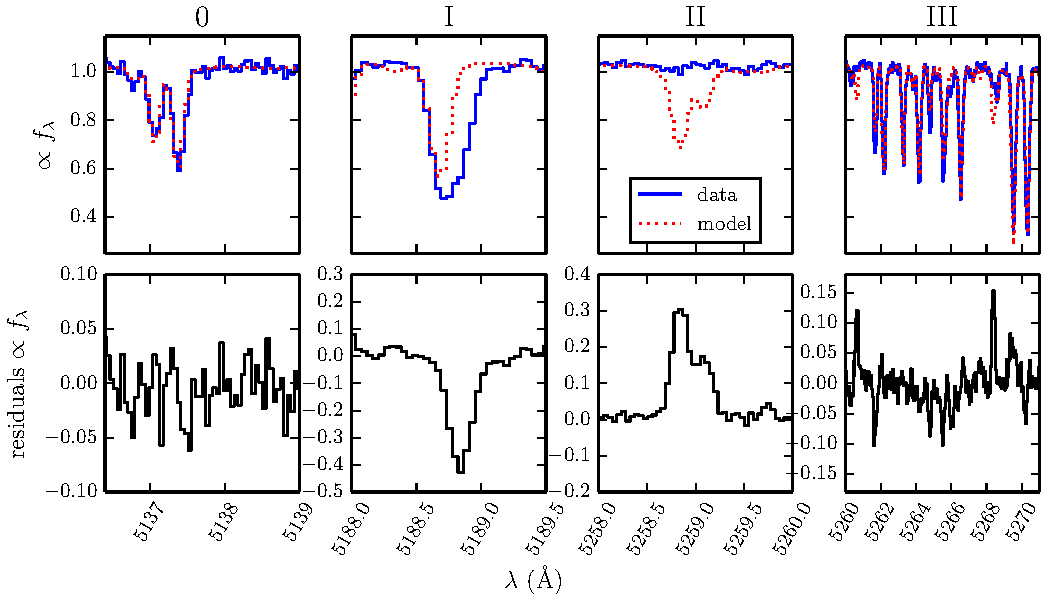
\includegraphics{figs/badlines.pdf}
  \caption{A collection of spectral lines induced by imperfect model fits.
    From left to right: \textbf{Class 0} The majority of spectral lines
    ($\gtrsim 60$\%) will have minor differences in strength between data and
    model spectrum, which produce low-amplitude correlations in the residuals
    on the length scale of the width of a typical spectral line.  \textbf{Class
    I}: Sometimes ($\lesssim 5$\% of all lines), a missing opacity source in
    the model (in this case a line-blended \ion{Ca}{1}) leaves a large, highly correlated
    patch of negative residuals.  \textbf{Class II}: Sometimes ($\lesssim 5$\%
    of all lines), an extraneous line in the model leaves a large, highly
    correlated patch of positive residual.  \textbf{Class III}: If the line strengths are
    substantially discrepant ($\lesssim 10$\% of all lines), there will be many
    correlated residuals of moderate amplitude.  The difficulty
    with class III lines is that for any specific line, there might exist a
    $\vstar$ that will fit the line, but there does not exist a $\vstar$ that
    will properly fit \emph{all} the lines.}
\label{fig:badlines}
\end{center}
\end{figure*}

However, the pixel residuals from a spectroscopic fit will often be correlated and will invalidate Equation~\ref{eqn:chi2}. These correlations arise because the CCD pixels of a spectrograph do not sample independent wavelengths of the spectrum. Instead, spectrographs are designed so that the LSF is properly sampled by at least a few pixels, meaning that adjacent pixels do not sample completely independent parts of the spectrum. Because of this, when a spectral feature differs between the model and the data it creates a residual which spans several adjacent data points. For a collection of correlated residuals produced by a typical spectroscopic fit, see Figure~\ref{fig:badlines}. 

\begin{figure*}[!htb]
\begin{center}
  $\vcenter{\hbox{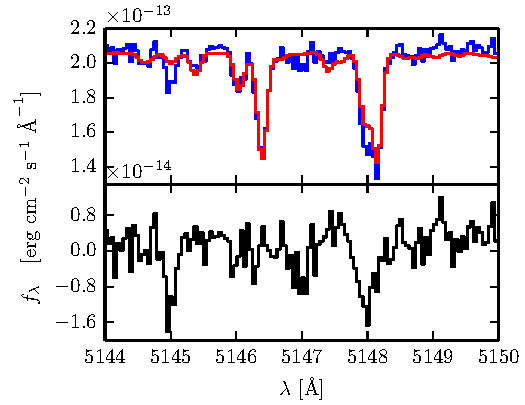
\includegraphics{figs/class0_residuals.pdf}}}$
  $\vcenter{\hbox{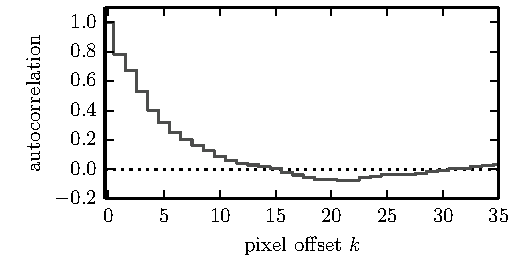
\includegraphics{figs/class0_autocorrelation.pdf}}}$
  \caption{\textbf{Left} The same residuals from Figure~\ref{fig:badlines}, panel 0, but shown at greater zoom to show the mildly covariant structure produced by slight mismatch between the data and model spectra.   
  \textbf{Right} The autocorrelation (Equation~\ref{eqn:autocorrelation}) of the residual sequence shown at left. Notice that there is significant correlation for offsets of $\sim 3 -4$ pixels.}
\label{fig:class0}
\end{center}
\end{figure*}

There is an important distinction between astrophysical or instrumental ``noise'' and the amplitude and correlation length of the residuals from a spectroscopic fit. Noise introduced to a spectrum by astrophysical or instrumental effects is generally uncorrelated with wavelength. This is because the arrival of each photon to the detector is a discrete event, and while photons are scattered by the LSF, the particular scattering direction of each photon is independent from any other photon. We can verify this by measuring the autocorrelation of residuals in a region of well-fit stellar continuum, and show that it is flat. However, when we compare two spectra that have many absorption lines, even small differences between the data and model spectra will produce correlated \emph{residuals}. We can verify this correlation by estimating the autocorrelation of the residuals
\begin{equation}
  \hat{\rho}\,(k) = \frac{1}{(n - k)\,\sigma^2} \sum_{i = 1}^{n - k} (R_i - \mu_R)\,(R_{i+k} - \mu_R)
  \label{eqn:autocorrelation}
\end{equation}
over a region of spectrum of length $n$. Figure~\ref{fig:class0} shows a general residual structure induced by slight model mismatch and the autocorrelation of this series. There is significant correlation on length scales of $\sim 3 -4$ pixels, which is also the typical width of a spectral line for this spectrum.

Although the correlation in the residuals is artificially induced by an
imperfect model fit rather than originating from a physical source of
correlated noise, we can treat these two effects as mathematically similar. By
using a non-trivial covariance matrix with off-diagonal terms we can describe
the small-scale covariance between pixel residuals shown in
Figures~\ref{fig:badlines}~and~\ref{fig:class0}. A non-diagonal covariance also
requires that we use  a likelihood function (Equation~\ref{eqn:lnprob}) which
uses a matrix product instead of a sum over independent pixels.

We seek to understand and parameterize the structure of covariance in the
spectroscopic residuals, because ignoring this complexity will bias the estimates of
the model parameters $\vt$. As a simple analogy, consider the fit of a straight
line to a dataset.  If the noise in the dataset is correlated, then adjacent
data points might be offset from the linear trend in the same direction by a
similar amount.  If the covariant structure of the noise is ignored, a simple
$\chi^2$ will treat these correlated offsets as part of the linear trend, which
will result in a biased determination of the slope and intercept of the line,
typically with uncertainties that are too small. We face a mathematically similar problem with 
correlated pixel residuals from a spectroscopic fit.

We parameterize the covariance structure using covariance kernels, taken from
the canon of Gaussian processes. Covariance kernels describe the covariance
between two pixels $\lambda_i$ and $\lambda_j$.  These kernels are analogous to
the cosmological two-point correlation function, where the distance
between two galaxies is used instead of wavelength of light.

\paragraph{Global and mildly covariant structure}
To account for the mild covariance structure shown in Figure~\ref{fig:class0},
which is generally low amplitude and has a correlation length of only a few
pixels but is present throughout the majority of the spectrum, we use a
\emph{stationary} covariance kernel. Stationary covariance kernels, also called \emph{radial basis functions}, satisfy the property that the
amount of correlation only depends on the distance between the two pixels $r$.  For spectra,
we map $r$ to the velocity difference between two pixels
\begin{equation}
  r\,(\lambda_i, \lambda_j) = \Delta v = \frac{c}{2} \left | \frac{\lambda_i 
   - \lambda_j}{ \lambda_i + \lambda_j} \right |
\end{equation}
Then the covariance kernel describes the expected covariance between pixel residuals
\begin{equation}
  k(\lambda_i, \lambda_j) =  \langle R_i \; R_j \rangle
  \label{eqn:expectation}
\end{equation}
In theory, we could chose from a variety of covariance kernels to parameterize this mildly covariant structure, as long as they satisfy the property that the degree of covariance smoothly declines with increasing radial distance. In practice, there are a few covariance kernels which are well-respected within the machine-learning community and frequently employed to parameterize covariance of this nature \citep{rw05}. We choose to use the \matern\ $\nu = 3/2$ kernel because it is one of the most commonly used kernels for this purpose and has an extensive history of use (cite?).
\begin{equation}
  k_{\nu = 3/2}(r,\, a,\, l) = a \left(1 + \frac{\sqrt{3} r}{l} \right ) \exp 
   \left (- \frac{\sqrt{3} r}{l} \right )
\end{equation}
This kernel is an exponential tapered by a polynomial, which makes for a smooth transition from small scale covariance to negligible covariance at longer scales. In order to ensure sparsity of the covariance matrix for computational efficiency, we
 taper the \matern\ kernel for compact support using a Hann window
\begin{equation}
  w\,(r,\, r_0) = \left \{ 
    \begin{array}{cc}
    0.5 + 0.5 \cos (\pi r/ r_0 ) & r \le r_0 \\
    0 & r > r_0\\
  \end{array}
  \right .
  \label{eqn:Hann}
\end{equation}
for a final covariance kernel of 
\begin{equation}
  k_{\rm global} (r,\, a,\, l,\, r_0) = w(r,\, r_0)\; k_{\nu = 3/2}(r,\, a,\, l) 
  \label{eqn:global}
\end{equation}
We add this covariance kernel to the independent pixel noise $\delta_{ij} \sigma_{ij}$ already present along
 the matrix diagonal, and introduce an additional parameter to allow a constant rescaling of the independent noise. Thus, each element of the covariance matrix is completely described by
\begin{equation}
  k(\lambda_i, \lambda_j |\, r,\, a,\, l,\, r_0,\, b) = k_{\rm global}(r, a, l, r_0) + b\,\delta_{ij} \sigma_{ij}
\end{equation}
Therefore, the \emph{hyperparameters} of this covariance kernel directly dictate the structure of the covariance matrix. By varying the hyperparameters, we can create a covariance matrix which accurately mimics the correlated structure of the pixel residuals. Most importantly, when the hyperparameters are correctly chosen to properly model this correlated structure, the \emph{likelihood function will be maximized} (Equation~\ref{eqn:prob}) while encapsulating the \emph{true uncertainty in the model-data fit}.
 
\begin{figure*}[!htb]
\begin{center}
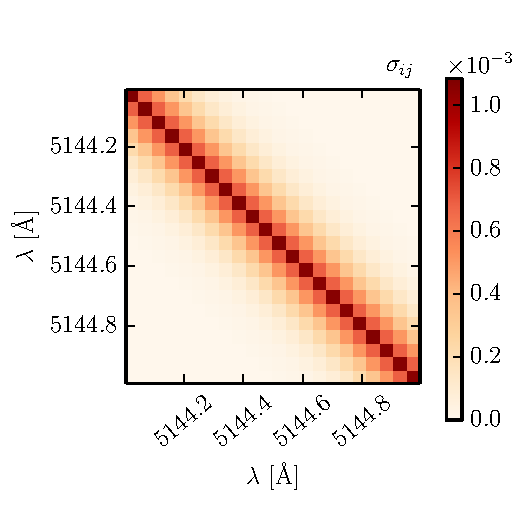
\includegraphics[width=0.4\textwidth]{figs/matern_matrix.pdf}
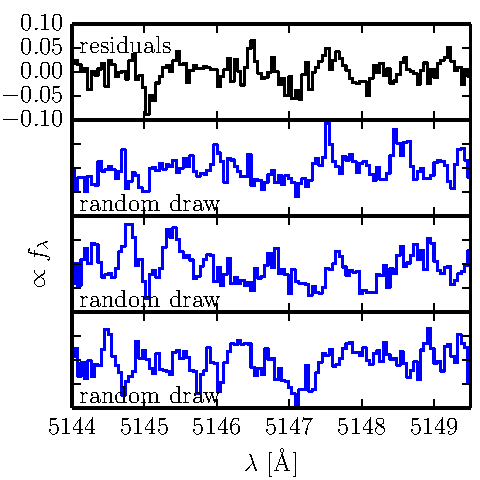
\includegraphics[width=0.4\textwidth]{figs/matern_draw.pdf}
\caption{\textbf{Left} Inset zoomed to show a small region of a typical covariance matrix, generated using the kernel in Equation~\ref{eqn:global}. There is a small degree of covariance in elements within a few pixels off the diagonal, which quickly tapers off such that the majority of the matrix remains sparse ($\sigma_{ij} = 0$). This matrix can be used to model spectrum which is correlated on a $\sim$few pixel scale.
\textbf{Right} To demonstrate that this matrix properly models the correlated structure of the residuals, we compare the residuals to random residuals generated from a multivariate normal distribution with this covariance matrix. Top: the same residuals shown in Figure~\ref{fig:class0}, plotted against three sets of simulated residuals. The amplitude and correlation length of the simulated residuals closely approximates the structure of the actual pixel residuals.}
\label{fig:matern}
\end{center}
\end{figure*}

The left panel of Figure~\ref{fig:matern} shows what the covariance matrix might look like for reasonable choices of the kernel hyperparameters. To verify that this covariance matrix indeed mimics the correlated structure seen in the residuals, we can draw a random vector of residuals $R_{\rm rand}$ from our noise model and compare it to the actual pixel residuals. Because we are using a multidimensional Gaussian as our likelihood function (Equation~\ref{eqn:prob}), we have assumed that the underlying residual structure in a spectroscopic fit is described by a multidimensional Gaussian. This is directly analogous to the implicit assumption of independent Gaussian noise when using a standard $\chi^2$ likelihood (Equation~\ref{eqn:chi2}). If one wished to compare the residuals that resulted from a $\chi^2$ fit to the noise in the data set, then one could simulate $R_{\rm rand}$ by drawing $N$ random samples from a univariate normal distribution with zero mean and variance $\sigma_i^2$. We can make the same test with our multidimensional Gaussian likelihood function, however in this case the mean is a vector $\vec{\mu} = 0$ with length $N$ and the variance is described by the covariance matrix $C$. The residual vector is then a random draw from this multivariate normal distribution 
\begin{equation}
  R_{\rm rand} \sim {\cal N}\left( \vec{\mu}=0,\, C\right)
\end{equation}
Functions to generate random samples from a multidimensional Gaussian are implemented in most numerical programming languages.

\paragraph{Specific line covariance} Even after the mildly covariant structure has been accounted for by the global covariance kernel (Equation~\ref{eqn:global}), there still exist a significant number large amplitude pixel residuals that are \emph{highly correlated}. These patches of large amplitude residuals are caused by incorrect lines like those in the class I, II, and III examples in Figure~\ref{fig:badlines}. To parameterize the covariance in a given patch of these residuals, we introduce an additional \emph{non-stationary} covariance kernel. In this context, non-stationary means that the degree of covariance explicitly depends on the values of $\lambda_i$ and $\lambda_j$, and not simply the distance between them, therefore we can now individually target the large residuals induced by the mismatch of a \emph{specific} spectral line.

Because the shape of a spectral line can be generally approximated by a Gaussian function, and the difference of two Gaussians with the same mean is also another Gaussian--the same shape of residuals that are shown in Figure~\ref{fig:badlines}--we use Equation~\ref{eqn:expectation} to design a new covariance kernel about the Gaussian function. If we expect the shape of the residuals to be a Gaussian function about the line center $\lambda_\mu$
\begin{equation}
  R(\lambda |\, a, \lambda_\mu, \sigma) = \frac{a}{\sqrt{2 \pi} \sigma} \exp \left (-\; \frac{r^2(\lambda, \lambda_\mu)}{2 \sigma^2} \right )
\end{equation}
then the Gaussian covariance kernel is
\begin{align}
k_{\rm G}(\lambda_i, \lambda_j |\, a, \lambda_\mu, \sigma) &= \langle R(\lambda_i)\; R(\lambda_j) \rangle \\
&= \frac{a^2}{2 \pi \sigma} \exp \left ( - \, \frac{r^2(\lambda_i, \lambda_\mu) 
    + r^2(\lambda_j, \lambda_\mu)}{2 \sigma^2}\right )
\end{align}
We again enforce compact support by tapering the kernel with a Hann window (Equation~\ref{eqn:Hann}), and so the covariance kernel for the highly correlated residuals induced by a poor line fit becomes
\begin{equation}
  k_{\rm line}(\lambda_i, \lambda_j |\, a, \lambda_\mu, \sigma, r, r_0) = w(r,\, r_0)\, k_{\rm G}(\lambda_i, \lambda_j |\, a, \lambda_\mu, \sigma)
  \label{eqn:line}
\end{equation}

\begin{figure*}[!htb]
\begin{center}
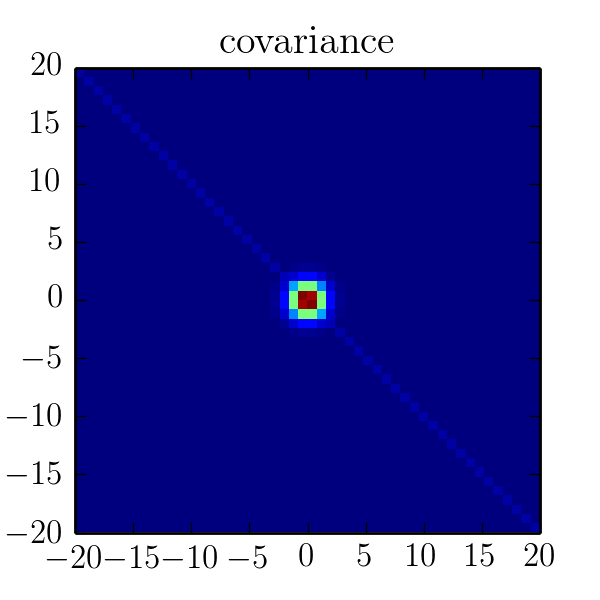
\includegraphics[width=0.4\textwidth]{figs/matrix_region_covariance.png}
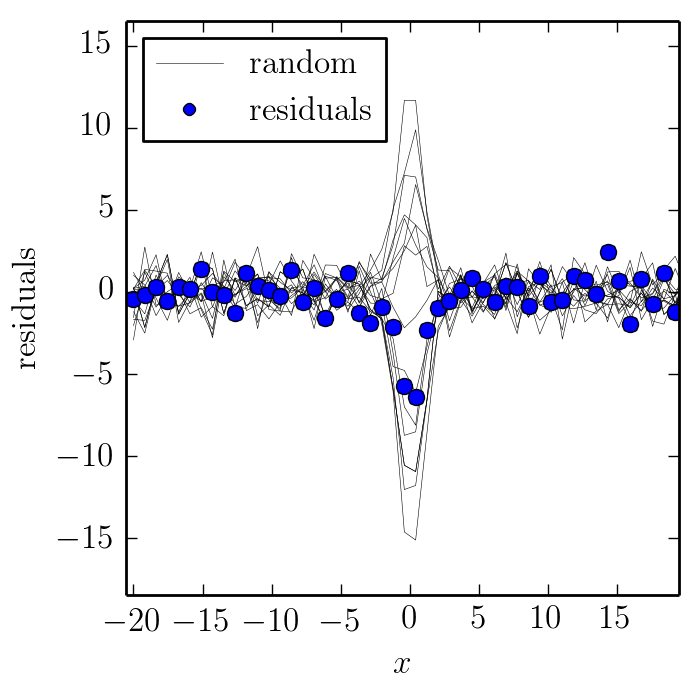
\includegraphics[width=0.4\textwidth]{figs/random_draw.png}
\caption{\textbf{Left} a covariance matrix generated with the region kernel.
\textbf{Right} general spectroscopic residuals near a mismatched stellar line
 overlaid with a sample draw using the covariance matrix, showing that the two
 look similar in structure and amplitude. 
\protect \todo{Similar improvements to
  Figure~\ref{fig:matern}.}}
\label{fig:region}
\end{center}
\end{figure*}

\todo{Similar paragraph about visualizing the covariance matrix, drawing
  samples. References to Figure~\ref{fig:region}.}

non-stationary kernel localizes increased variance to a specific
    spectral line

better than just masking out the region, since these contain info

here will be many sets of regions ($\sim$1-4\% of all lines might be
    covered by a region)
  
Covariance kernel parameters are parameters in our model that we explicitly sample for. There can be hyperparameters describing the \emph{population} of regions in a hierarchical model (mostly width, amplitude).


The benefit mainly comes from simply modelling these systematic residuals to
 begin with, since a model with covariance is far more likely than forcing the
 fit, and far more justified than masking regions which do not fit.

Where to draw the line between specific region and global covariance? When we reach some threshold, say three times the global amplitude?

\paragraph{M dwarf residual}
The squared exponential kernel is
\todo{Why do we use the squared exponential and not \matern?}
\begin{equation}
  k_{ \rm exp}(r, h) = \exp \left ( \frac{- r^2 }{2 h^2} \right )
\end{equation}
$h$ is a bandwidth. 
If $h$ is small, then there will be high-frequency structure. If $h$ is large,
 then only low-frequency structure will remain. 
We also use the Hann window to taper the kernel for compact support
\begin{equation}
  k(\lambda_i, \lambda_j | h, a, \mu, \sigma, r_0) = 
   w(r, r_0)\; k_{ \rm exp}(r, h) \; 
   k_{\rm G}(\lambda_i, \lambda_j | a, \mu, \sigma)
\end{equation}

\todo{Show how the kernel can accounts for complicated M dwarf structure where
 there is large, messy mismatch.}


\subsection{Exploring the posterior}
\label{subsec:MCMC}
Markov Chain Monte Carlo.

Gibbs sampler.
Sparse matrix.
Implemented using SuiteSparse and the Cholesky factorization, means that the RCR step can be computed quickly and reused.

Show figure using dfm/triangle.py that shows recovered stellar parameters and degeneracies. Separately for the regions.

\subsection{Applications}
\label{subsec:learning}
Learnt covariance structure can be used to correct the models.

\section{Tests}
\todo{Which tests to show?}


\bibliographystyle{yahapj}
\bibliography{stellarspectra}

\appendix

\begin{table}[!htb]
\begin{tabular}{ll}
\hline
\hline
Symbol & Description\\
\hline
\hline
$i$ & index specifying a pixel\\
$\lambda_i$ & wavelength corresponding to a given pixel $i$\\
$\vg$ & fundamental stellar parameters, $T_{\rm eff}, \log(g), \Z, \A$\\
  & that parameterize a synthetic spectrum from the grid\\
$\vpp$ & stellar parameters $v \sin i$, $v_z$, $A_V$, and $R^2/d^2$ that\\
  & are applied during ``post processing'' of the synthetic spectrum\\
$\vstar$ & $\{\vg,\vpp \}$\\
$\finst(\lambda)$ & data spectrum\\
$\fsynth(\lambda)$ & synthetic spectrum\\
$c_0, c_1, \ldots$ & Chebyshev polynomial coefficients for residual flux calibration\\
$\vN$ & the set of nuisance parameters composed of $\{c_0, c_1, \ldots, c_N\}$\\
$\vt$ & the parameters $\{\vg, \vpp, \vN\}$ that completely describe a model spectrum\\
$\fDi$ & data flux for a given pixel, $D(\lambda_i)$\\
$\fD$ & data vector comprised of all $\fDi$, $i = \{0, \ldots, N\}$\\
$\fMi$ & model flux for a given pixel, $M(\lambda_i | \vt)$\\
$\fM$ & model vector comprised of all $\fMi$, $i = \{0, \ldots, N\}$\\
$\sigma_i$ & Poisson noise for a given pixel $i$\\
$R_i$ & residuals $\fDi - \fMi$\\
$\fR$ & residual vector $\fD - \fM$\\
$C$ & covariance matrix\\
$k_{\rm global}$  & global covariance kernel\\
$k_{\rm region}$  & regional covariance kernel\\
\hline
\end{tabular}
\caption{Nomenclature used in this document.}
\label{tab:nomenclature}
\end{table}

This version of the paper was generated
 from a git repository available at \url{http://github.com/iancze/StellarSpectra/}
 with git hash \texttt{\githash\,(\gitdate)}.

\end{document}
